%!TEX root = ../main.tex

\subsubsection{CAN protocol}\label{sub:CAN_protocol}
Due to the requirements of the on-kart network, it is decided to formulate a new protocol specifically for this project. The requirements are listed below.\\
\textbf{On-kart network requirements}:
\begin{itemize}
	\item Simple and easy to learn.
	\item Support for 16 nodes.
	\item Broadcast data.
	\item Variable data length - beyond 8 bytes per message
	\item Expandable.
	\item Commands: Start/stop broadcasting 
	\item Commands can be send to specific or all nodes
\end{itemize}

The basic CAN framework is retained for this protocol, and the protocol is really just a naming convention for the message ID. 

\begin{figure}[h!]
	\centering
	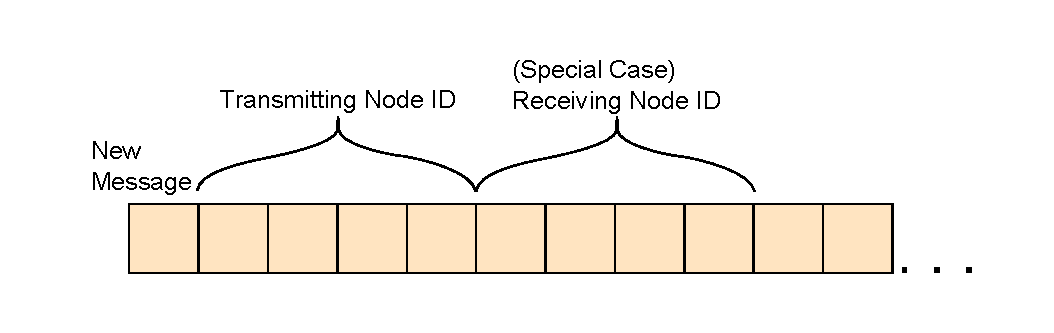
\includegraphics[width = 0.9\linewidth]{graphics/CAN_protocol_general_pdf}
	\caption{Naming convention for this high level protocol}
	\label{fig:CAN_protocol_general_pdf}
\end{figure}

The message ID is split in to three portions, as seen on figure~\ref{fig:CAN_protocol_general_pdf}.
The first bit is set to 1 if this is a new message.
If however the node needs to send more than 8 bytes in one package, this bit can be set to 0, thus blocking other nodes with higher priority.
The subsequent four bits indicate the transmitting node ID, which will allow up to 16 nodes. 
The last 6 bits of the message ID would contain an identifier for what the data portion of the frame contains.
This leaves 64 different message types for each node -- it is then the developers to utilize these the best. 
If more message types are needed, the CAN protocol supports extended identifier, which adds 18 bits of identifiers.
Each node will have a list of message IDs (10 bits), that it knows how to handle.
If a message is not on that list, the node will ignore it.\\

There are basically two types of nodes: The Wifi node acting a , and all other nodes.
Generally nodes can either produce data, and/or receive commands.
The Wifi node neither produces any kind of data nor receives commands, but it does receive data, and send out commands.
Therefore, there is a special case, for where the Wifi node is sending.
In this case, the subsequent four bits determines the recipient, leaving two bits for command type. 
For this part, command types are only "Start broadcasting" and "Stop broadcasting", but could be extended to for instance "Set parameter" or "Set value", where the data field will indicate which parameter, and what is's set to.\\

The four node IDs are:
\begin{table}[h!]
	\begin{tabular}{{l} {l}}
		Wifi node: & 0b0001 \\
		IMU node: & 0b0011 \\
		Sevcon node: & 0b0111 \\
		GPS node: & 0b1110
	\end{tabular}
\end{table}
The reason for this naming is, that the Wifi node acts as a commander for the, and it's commands need higher priority.
The IMU produces short data packages at a high rate, and the GPS node produces longer data packages at a lower rate. 
Therefore it is of less concern if the GPS message is delayed due to obstruction from other nodes. 